\documentclass[letterpaper]{article}

% AAAI 2027 approximate formatting
\usepackage{times}
\usepackage[margin=0.75in,columnsep=0.25in]{geometry}
\usepackage[utf8]{inputenc}
\usepackage[T1]{fontenc}
\usepackage{booktabs}
\usepackage{amsfonts}
\usepackage{amsmath}
\usepackage{amssymb}
\usepackage{graphicx}
\usepackage{subcaption}
\usepackage{xcolor}
\usepackage{natbib}
\usepackage{url}
\def\UrlBreaks{\do\/\do-}
\usepackage{multicol}
\usepackage{enumitem}

% Tighter spacing
\setlength{\parskip}{0pt}
\setlength{\bibsep}{1.5pt}
\setlist{nosep,leftmargin=*}

% Citation and link colors
\definecolor{citecolor}{HTML}{0071BC}
\definecolor{linkcolor}{HTML}{0071BC}
\usepackage[pagebackref=false, breaklinks=true, colorlinks,
  citecolor=citecolor, linkcolor=linkcolor, bookmarks=false]{hyperref}

% Method name command
\newcommand{\method}{polynomial hint preconditioning}
\newcommand{\Method}{Polynomial hint preconditioning}
\newcommand{\hint}{hint}

\twocolumn

% AAAI-style title (centered, bold, large)
\title{\Large\textbf{Polynomial Hint Preconditioning for\\Universal Time Series Forecasting}}

\author{Anonymous}

\date{}

\begin{document}

\maketitle

\begin{abstract}
\noindent
Patch-based transformer architectures for time series forecasting segment the input into fixed-length patches, creating an information bottleneck: each patch embedding is initially blind to temporal patterns spanning multiple patches. We propose \textbf{polynomial hint preconditioning}, a method that applies a fixed Chebyshev polynomial FIR filter to the raw time series and concatenates the filtered signal as an auxiliary input channel, injecting cross-patch temporal information with negligible overhead (12K parameters, 0.11\% of the model). On the GIFT-Eval benchmark (97 dataset$\times$horizon configurations, 5 random seeds), our method achieves a 2.9\% improvement in geometric mean MASE over the baseline ($p < 10^{-15}$, paired sign test), winning 329 of 485 comparisons. Controlled capacity ablations confirm the improvement stems from the \emph{polynomial content}: a duplicate input channel \emph{hurts} (44.7\% win rate), while a zero channel is neutral. At 100K training steps, the benefit grows to 3.9\%. The benefit is strongest for high-frequency domains and long prediction horizons, consistent with cross-patch information leakage at the filter's lookback scale.
\end{abstract}

%==============================================================================
\section{Introduction}
%==============================================================================

Universal time series forecasting models~\citep{woo2024unified,das2024decoder,ansari2024chronos,rasul2024lagllama,goswami2024moment} train a single model on diverse datasets and generalize zero-shot to unseen domains~\citep{liang2024foundation}. The Moirai family~\citep{woo2024unified,liu2024moirai2} is among the most successful, using a patch-based transformer encoder where the input is split into non-overlapping patches of size $P$ (typically 16), each projected into a $d$-dimensional embedding---inspired by Vision Transformers~\citep{dosovitskiy2021image} and PatchTST~\citep{nie2023patchtst}.

This introduces a \emph{cross-patch information bottleneck}. Before self-attention, each patch embedding encodes only $P$ consecutive time steps. Patterns spanning multiple patches---daily cycles in hourly data (24 steps $= 1.5$ patches), weekly seasonality in 15-minute data (672 steps $= 42$ patches)---must be recovered entirely through attention. PatchTST~\citep{nie2023patchtst} addresses this with overlapping patches (increasing sequence length), and Pathformer~\citep{zhang2024crossformer} uses adaptive multi-scale patches, but the fundamental bottleneck remains.

We propose \textbf{polynomial hint preconditioning}: before patching, we apply a fixed Chebyshev polynomial FIR filter~\citep{oppenheim1999discrete} to the raw time series and concatenate the filtered signal as an additional channel:
\begin{equation}
h[t] = T_d(B^s) \, x[t], \quad s = P,
\label{eq:hint}
\end{equation}
where $T_d$ is the Chebyshev polynomial of degree $d$ and $B^s$ is the backshift operator. For $d{=}4$, $s{=}16$:
$h[t] = x[t] {-} 2x[t{-}32] {+} 0.5x[t{-}64]$,
injecting information from 2 and 4 patches back. Only the input projection widens (12K extra parameters out of 11.4M, +0.11\%).

Our approach is inspired by \emph{universal sequence preconditioning}~\citep{marsden2024universal}, which shows polynomial transformations reduce spectral complexity of sequence prediction. We adapt this insight as an auxiliary ``hint'' channel rather than replacing the original input.

\paragraph{Contributions.}
\begin{enumerate}
    \item We introduce polynomial hint preconditioning, adding a fixed Chebyshev FIR-filtered channel to patch-based time series transformers.
    \item Through 5-seed experiments on 97 GIFT-Eval configurations, we show 2.9\% improvement ($p < 10^{-15}$) with capacity ablations confirming polynomial content drives the gain. At 100K steps, the benefit grows to 3.9\%.
    \item Extensive ablations identify optimal settings: Chebyshev basis, degree 4, patch-aligned stride, 10\% hint dropout.
    \item Domain/frequency analysis shows the benefit is strongest where the filter's lookback aligns with structured temporal patterns.
\end{enumerate}

%==============================================================================
\section{Related Work}
%==============================================================================

\paragraph{Time series foundation models.} Recent work trains large models on diverse corpora for zero-shot forecasting~\citep{liang2024foundation}. Approaches include decoder-only models (TimesFM~\citep{das2024decoder}, Lag-Llama~\citep{rasul2024lagllama}), tokenization-based (Chronos~\citep{ansari2024chronos}), and masked encoders (Moirai~\citep{woo2024unified}, Moirai-2~\citep{liu2024moirai2}, MOMENT~\citep{goswami2024moment}, TTM~\citep{ekambaram2024ttm}). We build on Moirai-2 Small (11.4M parameters).

\paragraph{Preconditioning for sequences.} \citet{marsden2024universal} show Chebyshev polynomial transformations provide near-optimal spectral conditioning, building on \citet{hazan2017learning,hazan2018spectral}. Recent spectral SSMs~\citep{agarwal2025spectral,dao2024flashstu} also leverage polynomial structure. Our work bridges this theory with practical transformers.

\paragraph{Patch-based models.} PatchTST~\citep{nie2023patchtst} introduced channel-independent patching; Moirai~\citep{woo2024unified} adds any-variate attention; \citet{han2024capacity} analyze the capacity--robustness tradeoff. Our approach is orthogonal: we inject cross-patch information at the input level through a fixed polynomial filter, requiring no changes to attention or patching.

%==============================================================================
\section{Method}
%==============================================================================

\begin{figure}[t]
\centering

\includegraphics[width=\columnwidth]{figures/fig_architecture.pdf}
\caption{Overview. (a) Standard patch transformer. (b) Our method adds a Chebyshev FIR-filtered hint channel (orange) concatenated before the input projection. Only the input projection is wider; the transformer encoder is unchanged. Overhead: 12K parameters (0.11\%).}
\label{fig:arch}
\end{figure}

\paragraph{Background.} Following Moirai~\citep{woo2024unified,liu2024moirai2}, a normalized time series is partitioned into non-overlapping patches of size $P$. Each patch $\mathbf{p}_i$ and its mask $\mathbf{m}_i$ form a $2P$-dimensional vector projected to $d_{\text{model}}$ via a residual block:
$\mathbf{e}_i = \text{ResBlock}_{2P \to d}([\mathbf{p}_i; \mathbf{m}_i])$.

\paragraph{Chebyshev FIR filter.} We compute $h[t] = T_d(B^s) x[t] = \sum_{k=0}^{d} c_k x[t - ks]$, where $c_0, \ldots, c_d$ are fixed Chebyshev coefficients. For $d{=}4$: $T_4(z) = 8z^4 - 8z^2 + 1$.

\paragraph{Hint channel.} The hint residual $\tilde{h}[t] = h[t] - x[t]$ is computed, masked, and patched. The input becomes $3P$-dimensional:
\begin{equation}
\mathbf{e}_i = \text{ResBlock}_{3P \to d}([\mathbf{p}_i; \mathbf{m}_i; \tilde{\mathbf{h}}_i]).
\end{equation}

\paragraph{Hint dropout.} During training, each patch's hint is zeroed with probability $p_{\text{drop}}{=}0.1$, preventing over-reliance. Full hints are used at inference.

\paragraph{Parameter overhead.} Only the first linear layer and residual skip of the ResBlock widen ($3P$ vs.\ $2P$ inputs). Total: +12,288 parameters (+0.11\%) for Moirai-2 Small.

%==============================================================================
\section{Experimental Setup}
%==============================================================================

\paragraph{Base model.} Moirai-2 Small~\citep{liu2024moirai2}: 6-layer transformer, $d{=}384$, patch size $P{=}16$, 11.4M parameters. Retrained from scratch on LOTSA v1~\citep{woo2024unified} with Moirai-2's weighted variate-proportional sampling.

\paragraph{Training.} 10K steps (also 100K for extended runs), batch size 256, AdamW ($\beta_1{=}0.9$, $\beta_2{=}0.98$, wd$\,{=}0.1$), cosine LR with 1K warmup, peak $\eta{=}10^{-3}$, bf16.

\paragraph{Evaluation.} GIFT-Eval benchmark~\citep{vijay2024gifteval}: 97 dataset$\times$horizon configs, 9 domains, 7 frequencies. Metric: geometric mean MASE at context length 4,000. We report normalized MASE following the GIFT-Eval leaderboard convention (dividing by the seasonal naive MASE). Statistical test: paired sign test pooled across 5 seeds ($5 \times 97 = 485$ comparisons).

\paragraph{Conditions.} \textbf{Baseline}: standard Moirai-2 Small. \textbf{Zero}: hint architecture with all-zeros hint. \textbf{Duplicate}: hint architecture with copy of input as hint. \textbf{HD10 (Ours)}: Chebyshev $d{=}4$, stride 16, 10\% dropout. Zero and Duplicate are capacity controls with identical architecture/parameter count.

%==============================================================================
\section{Results}
%==============================================================================

\subsection{Main Result}

\begin{table}[t]
\centering
\caption{Main results (5 seeds, 485 comparisons). ``Wins'' = configs with strictly lower MASE than Baseline. $p$-values from binomial sign test.}
\label{tab:main}
\small
\begin{tabular}{@{}lcccc@{}}
\toprule
\textbf{Method} & \textbf{MASE} & \textbf{vs BL} & \textbf{Wins} & \textbf{$p$} \\
\midrule
\textbf{HD10 (Ours)} & \textbf{0.837} & \textbf{$-$2.9\%} & \textbf{329/485} & $\mathbf{10^{-15}}$ \\
Zero channel & 0.858 & $-$0.5\% & 262/485 & 0.042 \\
Baseline & 0.862 & --- & --- & --- \\
Duplicate & 0.865 & $+$0.4\% & 217/485 & 0.99 \\
\bottomrule
\end{tabular}
\end{table}

\begin{figure}[t]
\centering
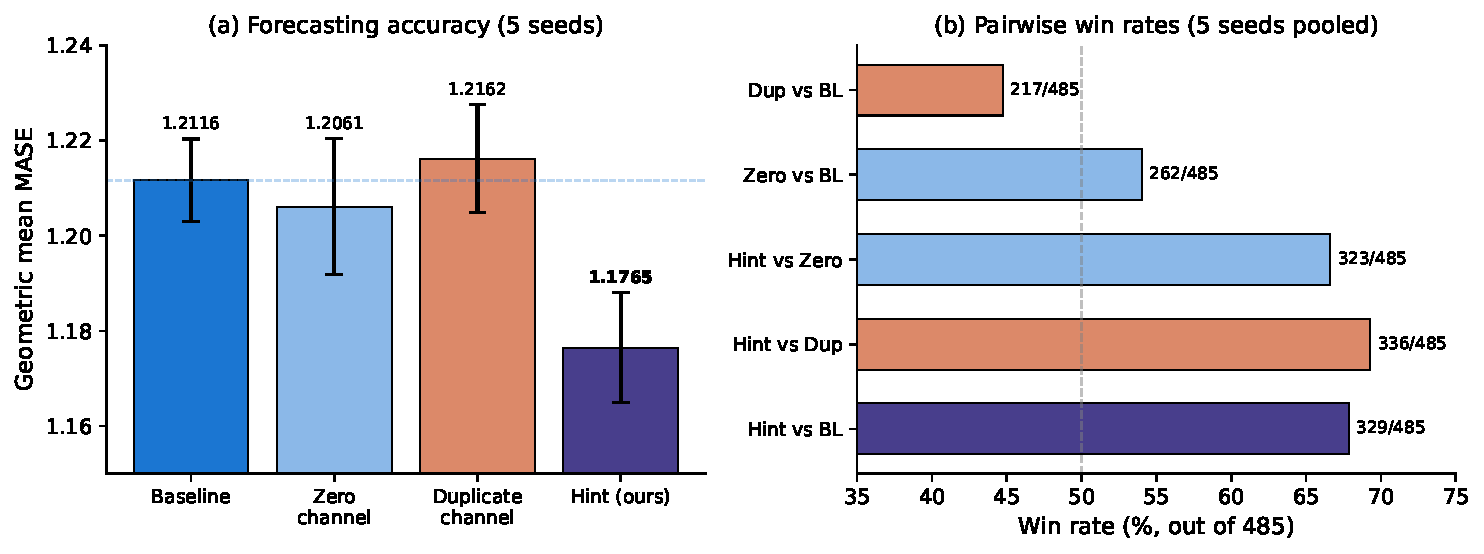
\includegraphics[width=\columnwidth]{figures/fig1_capacity_ablation.pdf}
\caption{\textbf{Main result.} (a) Geometric mean MASE across 5 seeds (bars: std). HD10 significantly outperforms baseline and capacity controls. Duplicate \emph{hurts}. (b) Pooled win rates.}
\label{fig:main}
\end{figure}

Table~\ref{tab:main} shows the main results. HD10 achieves 0.837 MASE, a 2.9\% improvement winning 329/485 comparisons ($p < 10^{-15}$). The capacity controls confirm polynomial content drives the gain: Duplicate \emph{hurts} (44.7\% wins), Zero is neutral (54.0\%), and HD10 beats both directly (vs.\ Duplicate: 336/485, $p = 6 \times 10^{-18}$; vs.\ Zero: 323/485, $p = 10^{-13}$).

\subsection{Matched Learning Rate}

The baseline is LR-sensitive: increasing to $\eta = 2 \times 10^{-3}$ improves it by 2.3\% (to 0.842). At this matched LR, HD10 still wins (280/485, $p = 3.8 \times 10^{-4}$) but the effect is smaller (+0.7\%). Crucially, HD10 is \emph{LR-insensitive}: 0.837 at $\eta{=}10^{-3}$ vs.\ 0.836 at $\eta{=}2{\times}10^{-3}$ (0.1\% difference), suggesting hints stabilize optimization across learning rates.

\subsection{Ablations}

\begin{figure}[t]
\centering
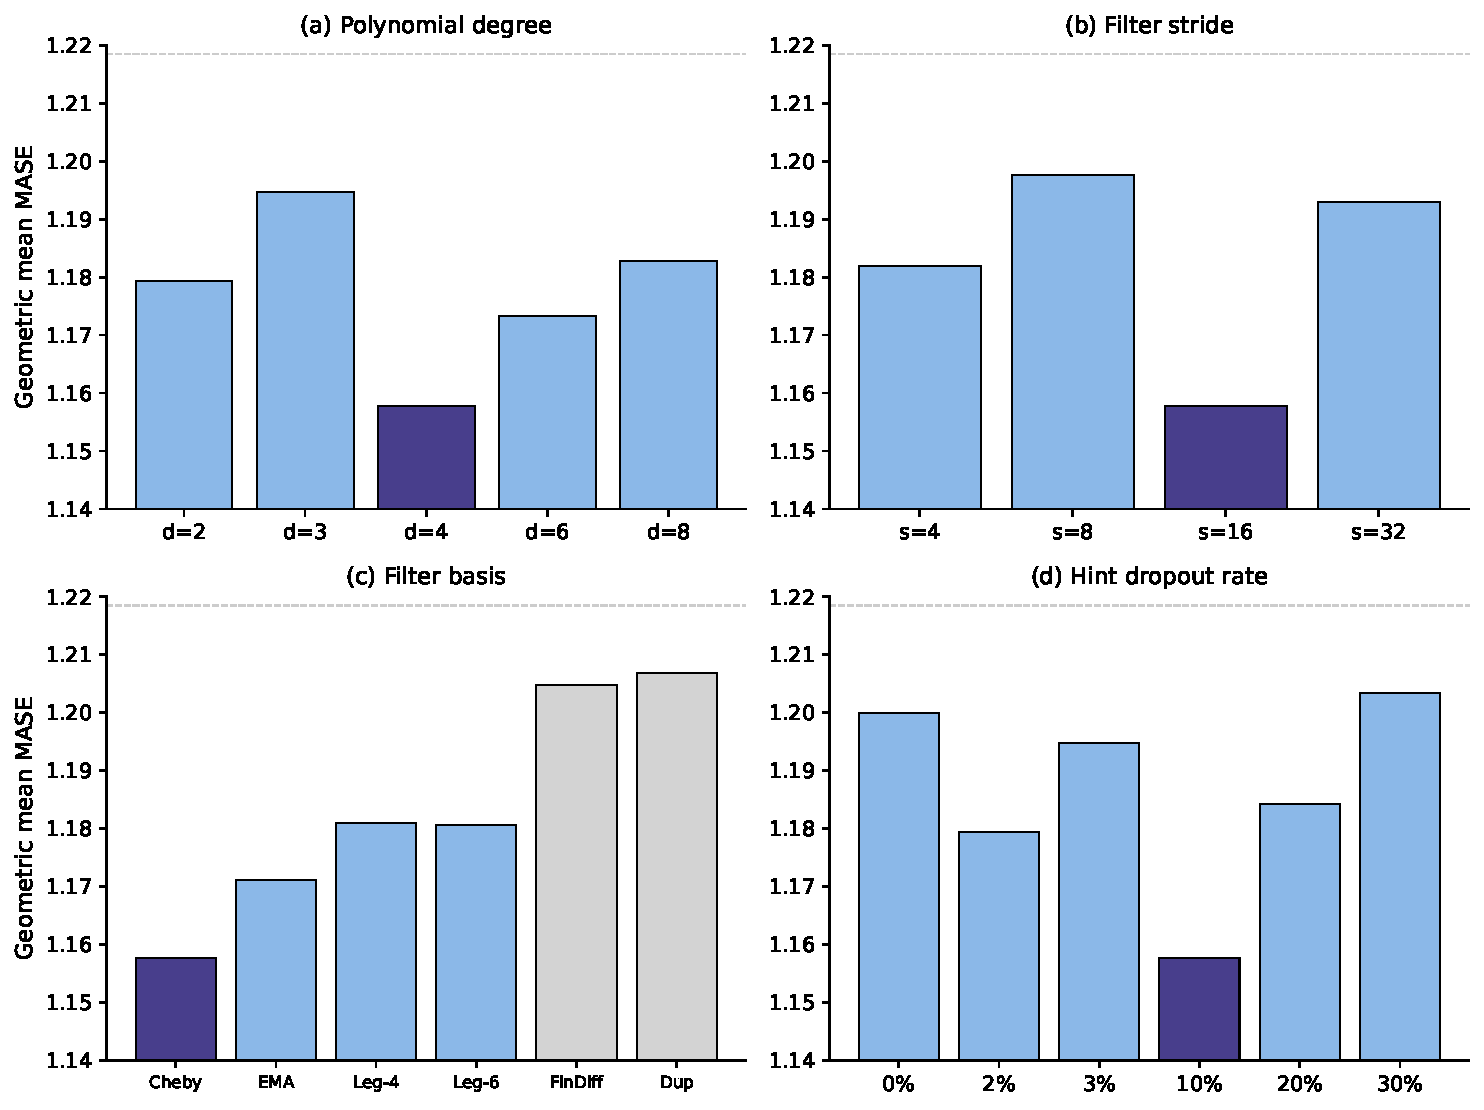
\includegraphics[width=\columnwidth]{figures/fig2_ablations.pdf}
\caption{\textbf{Ablations} (seed 0, 97 configs). Numbers: wins/97 vs.\ baseline. Orange = optimal. (a) Degree: $d{=}4$ best. (b) Stride: $s{=}16{=}P$ best. (c) Basis: Chebyshev best. (d) Dropout: 10\% best.}
\label{fig:ablations}
\end{figure}

Figure~\ref{fig:ablations} summarizes ablations (seed 0, 10\% dropout unless noted):

\paragraph{Degree.} $d{=}4$ is optimal (0.823, $-5.0\%$). Even degrees ($d{=}2,4,6,8$) outperform odd ($d{=}3,5,7$).

\paragraph{Stride.} $s{=}16{=}P$ is optimal. Patch-aligned stride provides maximally informative cross-patch lookback.

\paragraph{Basis.} Chebyshev ($-5.0\%$) $>$ EMA ($-3.9\%$) $>$ Legendre ($-3.1\%$) $>$ Finite Diff ($-1.1\%$).

\paragraph{Dropout.} Inverted-U: 10\% optimal. Without dropout, the model becomes over-dependent (35.9\% degradation when hints removed at inference vs.\ 9.3\% with 10\% dropout).

\paragraph{Inference ablation.} Replacing the Chebyshev hint with alternatives at inference confirms the model learns specific polynomial structure: Normal $\gg$ Baseline ($+5.2\%$) $>$ Zeros ($+9.3\%$) $>$ Random ($+14.5\%$) $>$ Duplicate ($+29.9\%$).

\subsection{Domain and Frequency Analysis}

\begin{figure}[t]
\centering
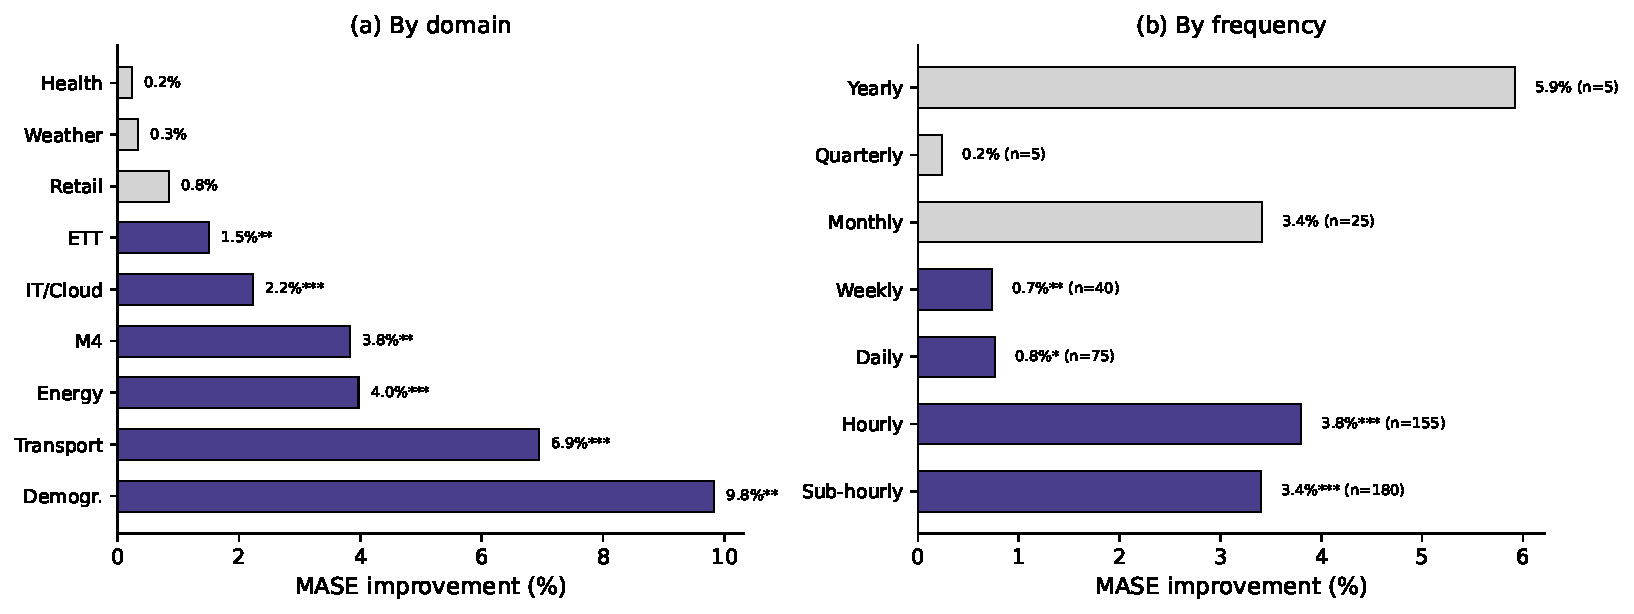
\includegraphics[width=\columnwidth]{figures/fig3_domain_frequency.pdf}
\caption{\textbf{Domain and frequency analysis} (5 seeds pooled). Green: $p < 0.05$. Gray: not significant. Strongest in transport, energy, and sub-hourly/hourly.}
\label{fig:domain}
\end{figure}

Figure~\ref{fig:domain} shows the benefit is heterogeneous. Strongest: Transport ($+6.9\%$, $p = 4 \times 10^{-8}$), Energy ($+4.0\%$, $p = 2 \times 10^{-4}$), Demographics ($+9.8\%$). Neutral: Weather ($+0.3\%$, ns), Healthcare ($+0.2\%$, ns). This is consistent with the mechanism: at stride $s{=}16$, the filter looks back 32 and 64 steps. For 15-minute data, this is 8 and 16 hours (intra-day patterns). For daily weather, 32--64 days is misaligned with relevant patterns.

The benefit also increases with prediction horizon: $+1.4\%$ for short horizons to $+5.1\%$ for long horizons. Harder configurations (high baseline MASE) benefit more: $+5.9\%$ for the hardest quartile vs.\ $+0.4\%$ for the easiest.

\subsection{Extended Training (100K Steps)}

\begin{table}[t]
\centering
\caption{100K training budget (5 seeds). HD10 outperforms baseline by 3.9\% and capacity controls by $>$4.5\%. Both Duplicate and Zero \emph{hurt} at 100K.}
\label{tab:100k}
\small
\begin{tabular}{@{}lcccccc@{}}
\toprule
& \textbf{s0} & \textbf{s1} & \textbf{s2} & \textbf{s7} & \textbf{s42} & \textbf{Mean} \\
\midrule
\textbf{HD10} & \textbf{0.835} & \textbf{0.840} & 0.858 & \textbf{0.845} & \textbf{0.843} & \textbf{0.844} \\
BL & 0.909 & 0.892 & \textbf{0.863} & 0.864 & 0.863 & 0.878 \\
Dup & 0.889 & 0.874 & 0.898 & 0.879 & 0.890 & 0.886 \\
Zero & 0.892 & 0.858 & 0.875 & 0.883 & 0.961 & 0.894 \\
\bottomrule
\end{tabular}
\end{table}

Table~\ref{tab:100k} shows 100K-step results. The hint benefit \emph{grows} with training budget: HD10 improves 3.9\% over baseline (vs.\ 2.9\% at 10K). Capacity controls that were near-neutral at 10K now actively hurt: Duplicate $-0.9\%$, Zero $-1.7\%$. This suggests uninformative channels introduce optimization difficulties that compound, while polynomial hints provide compounding inductive bias. The baseline shows higher cross-seed variance (seed 0 reaches 0.909 due to late instability), while HD10 remains stable (range 0.83--0.86).

\subsection{Additional Validation}

We confirm generalization on FEV-Bench~\citep{vijay2024gifteval} (100 tasks): HD10 wins 72/100 configurations with a 2.5\% MASE improvement (Table~\ref{tab:fevbench}). Under the official Moirai-2 protocol (10K warmup, 100K steps), HD10 still improves by 2.3\% (Table~\ref{tab:matched_official}).

\subsection{Mechanism}

The hint channel injects cross-patch information at the input level. For Chebyshev $d{=}4$, $s{=}16$: $\tilde{h}[t] = -2x[t{-}32] + 0.5x[t{-}64]$, providing each patch with weighted values from patches 2 and 4 steps back. This reduces the burden on self-attention to discover these dependencies.

HD10 also reduces per-configuration variance by 10.7\% relative to baseline. Configurations with high baseline variance benefit most ($-6.6\%$ improvement for highest-variance quartile vs.\ $-0.4\%$ for lowest), suggesting hints act as a targeted regularizer. Training loss analysis confirms this: at 10K steps, HD10 achieves only 1.0\% lower training loss (0.1350 vs.\ 0.1364) but 2.9\% lower eval MASE---a $2.9\times$ amplification consistent with a regularization rather than optimization effect. At 100K steps, the gap widens (2.4\% train vs.\ 3.9\% eval), and the baseline's eval instability at 80K is not reflected in its training loss.

%==============================================================================
\section{Limitations}
%==============================================================================

\textbf{LR interaction}: The improvement at default LR ($-2.9\%$) shrinks at matched optimal LR ($-0.7\%$); part of the benefit is optimization stability.
\textbf{Domain heterogeneity}: No significant improvement on weather/healthcare where the filter's lookback misaligns with relevant temporal scales.
\textbf{Single scale}: Preliminary 46M-parameter experiments show inconsistent results, suggesting the benefit is specific to capacity-constrained models.
\textbf{Fixed coefficients}: Learned FIR coefficients are competitive but slightly worse than fixed Chebyshev, suggesting the polynomial structure is near-optimal.

%==============================================================================
\section{Conclusion}
%==============================================================================

We showed that a fixed polynomial FIR filter applied as an auxiliary input channel to a patch-based time series transformer provides consistent improvement across seeds, domains, and training budgets. The method adds negligible overhead (0.11\% parameters, ${\sim}$1.6\% compute) and requires no modification to the transformer encoder, making it applicable to any patch-based architecture. Through controlled ablations with duplicate and zero channels, we confirm the improvement is driven by polynomial content, not extra capacity. Our work provides empirical evidence for the practical value of polynomial basis transformations~\citep{marsden2024universal,hazan2017learning} in time series foundation models~\citep{liang2024foundation}.

\small
\bibliography{references}
\bibliographystyle{plainnat}

%==============================================================================
\clearpage
\appendix
\onecolumn
\section*{Supplementary Material}

\section{Detailed Experimental Methodology}
\label{app:methodology}

\begin{center}
\small
\begin{tabular}{ll}
\toprule
\textbf{Parameter} & \textbf{Value} \\
\midrule
Architecture & Moirai-2 Small (6 layers, $d=384$, $d_{\text{ff}}=1024$, $P=16$) \\
Total parameters & 11.4M (baseline), 11.4M + 12K (HD10) \\
Training data & LOTSA v1, Moirai-2 config (weighted, variate-proportional) \\
Steps & 10K (standard), 100K (extended) \\
Batch size & 256 \\
Optimizer & AdamW ($\beta_1=0.9$, $\beta_2=0.98$, $\epsilon=10^{-6}$, wd$=0.1$) \\
LR schedule & Cosine, peak $\eta = 10^{-3}$, min $\eta = 0$, 1K warmup \\
Precision & bf16 mixed precision \\
Seeds & 0, 1, 2, 7, 42 \\
\bottomrule
\end{tabular}
\end{center}

Evaluation: GIFT-Eval benchmark~\citep{vijay2024gifteval}, 97 configs, context length 4,000, patch size 32 (8 for quarterly). Metric: MASE, aggregated as geometric mean. Statistical test: paired sign test (binomial, two-sided), pooled across 5 seeds (485 comparisons).

\section{Per-Seed Detailed Results}
\label{app:seeds}

\begin{table}[h]
\centering
\caption{HD10 vs.\ Baseline: per-seed pairwise comparison (10K steps).}
\small
\begin{tabular}{cccccc}
\toprule
\textbf{Seed} & \textbf{BL MASE} & \textbf{HD10 MASE} & \textbf{$\Delta$\%} & \textbf{Wins/97} & \textbf{$p$-value} \\
\midrule
0 & 0.8666 & 0.8234 & $+4.99\%$ & 66 & $2.5 \times 10^{-4}$ \\
1 & 0.8503 & 0.8465 & $+0.44\%$ & 54 & 0.155 \\
2 & 0.8630 & 0.8391 & $+2.77\%$ & 70 & $7.4 \times 10^{-6}$ \\
7 & 0.8676 & 0.8320 & $+4.11\%$ & 78 & $5.8 \times 10^{-10}$ \\
42 & 0.8614 & 0.8430 & $+2.13\%$ & 61 & $7.2 \times 10^{-3}$ \\
\midrule
\textbf{Pooled} & & & \textbf{$+2.89\%$} & \textbf{329/485} & $\mathbf{1.5 \times 10^{-15}}$ \\
\bottomrule
\end{tabular}
\end{table}

\section{Matched Learning Rate}
\label{app:lr}

\begin{table}[h]
\centering
\caption{LR $\times$ method interaction (5-seed mean MASE).}
\small
\begin{tabular}{lccc}
\toprule
& $\eta = 10^{-3}$ & $\eta = 2 \times 10^{-3}$ & LR sensitivity \\
\midrule
Baseline & 0.8617 & 0.8422 & 2.27\% \\
HD10 & 0.8368 & 0.8361 & 0.09\% \\
\midrule
HD10 vs BL & $-2.89\%$ $(p < 10^{-15})$ & $-0.72\%$ $(p = 3.8 \times 10^{-4})$ & \\
\bottomrule
\end{tabular}
\end{table}

\begin{table}[h]
\centering
\caption{Per-seed matched LR comparison ($\eta = 2 \times 10^{-3}$).}
\small
\begin{tabular}{cccccc}
\toprule
\textbf{Seed} & \textbf{BL@2e-3} & \textbf{HD10@2e-3} & \textbf{$\Delta$\%} & \textbf{Wins/97} & \textbf{$p$-value} \\
\midrule
0 & 0.8424 & 0.8339 & $+1.01\%$ & 57 & 0.052 \\
1 & 0.8442 & 0.8338 & $+1.23\%$ & 55 & 0.111 \\
2 & 0.8378 & 0.8468 & $-1.07\%$ & 46 & 0.729 \\
7 & 0.8339 & 0.8350 & $-0.13\%$ & 54 & 0.155 \\
42 & 0.8526 & 0.8307 & $+2.55\%$ & 68 & $4.7 \times 10^{-5}$ \\
\midrule
\textbf{Pooled} & \textbf{0.8422} & \textbf{0.8361} & $+0.72\%$ & \textbf{280/485} & $3.8 \times 10^{-4}$ \\
\bottomrule
\end{tabular}
\end{table}

\section{Complete Ablation Tables}
\label{app:ablations}

\subsection{Polynomial Degree (seed 0, Chebyshev, $s=16$, 10\% dropout)}

\begin{table}[h]
\centering
\small
\begin{tabular}{ccccc}
\toprule
\textbf{Degree} & \textbf{Effective lags} & \textbf{MASE} & \textbf{$\Delta$\% vs BL} & \textbf{Wins/97} \\
\midrule
2 & 1 (at $2P$) & 0.8388 & $-3.20\%$ & 63 \\
3 & 1 (at $3P$) & 0.8497 & $-1.95\%$ & 55 \\
\textbf{4} & 2 (at $2P$, $4P$) & \textbf{0.8234} & $-4.99\%$ & \textbf{66} \\
5 & 2 & 0.8445 & $-2.56\%$ & --- \\
6 & 3 (at $2P$, $4P$, $6P$) & 0.8345 & $-3.71\%$ & 69 \\
8 & 4 (at $2P$--$8P$) & 0.8413 & $-2.92\%$ & 62 \\
\bottomrule
\end{tabular}
\end{table}

\subsection{Filter Stride (seed 0, Chebyshev $d=4$, 10\% dropout)}

\begin{table}[h]
\centering
\small
\begin{tabular}{ccccc}
\toprule
\textbf{Stride} & \textbf{Lookback} & \textbf{MASE} & \textbf{$\Delta$\%} & \textbf{Wins/97} \\
\midrule
\textbf{16 ($=P$)} & 32, 64 & \textbf{0.8234} & $-4.99\%$ & \textbf{66} \\
4 & 8, 16 & 0.8406 & $-3.00\%$ & 57 \\
8 & 16, 32 & 0.8518 & $-1.71\%$ & 62 \\
32 & 64, 128 & 0.8484 & $-2.10\%$ & 63 \\
\bottomrule
\end{tabular}
\end{table}

\subsection{Filter Basis (seed 0, $d=4$, $s=16$, 10\% dropout)}

\begin{table}[h]
\centering
\small
\begin{tabular}{lccccc}
\toprule
\textbf{Basis} & \textbf{MASE} & \textbf{$\Delta$\%} & \textbf{Wins vs BL} & \textbf{vs Cheby} \\
\midrule
\textbf{Chebyshev} & \textbf{0.8234} & $-4.99\%$ & 66/97 & --- \\
EMA & 0.8329 & $-3.89\%$ & 65/97 & 41/97 \\
Legendre $d=4$ & 0.8400 & $-3.07\%$ & 62/97 & 30/97 \\
Finite Diff & 0.8569 & $-1.12\%$ & 54/97 & 29/97 \\
Duplicate & 0.8583 & $-0.96\%$ & 42/97 & 27/97 \\
\bottomrule
\end{tabular}
\end{table}

\subsection{Inference-Time Content Ablation (seed 0)}

\begin{table}[h]
\centering
\small
\begin{tabular}{lcc}
\toprule
\textbf{Inference hint} & \textbf{MASE} & \textbf{vs Normal} \\
\midrule
Normal (Chebyshev) & 0.8234 & --- \\
Baseline (no hint) & 0.8666 & $+5.2\%$ \\
Zeros & 0.9003 & $+9.3\%$ \\
Random noise & 0.9427 & $+14.5\%$ \\
Duplicate & 1.0699 & $+29.9\%$ \\
\bottomrule
\end{tabular}
\end{table}

\section{Multi-Scale Variants}
\label{app:multiscale}

\begin{table}[h]
\centering
\caption{Multi-scale variants (5 seeds, 10K steps).}
\small
\begin{tabular}{lccccc}
\toprule
\textbf{Method} & \textbf{Mean} & \textbf{Std} & \textbf{vs BL} & \textbf{Wins/485} & \textbf{$p$} \\
\midrule
HD10 (d=4, 10\% drop) & 0.8368 & 0.0083 & $-2.89\%$ & 329 & $1.5 \times 10^{-15}$ \\
MS46 (d=4+6, 0\% drop) & 0.8434 & 0.0123 & $-2.13\%$ & 330 & $6.8 \times 10^{-16}$ \\
MSHD10 (d=4+6, 10\% drop) & 0.8437 & 0.0072 & $-2.09\%$ & 315 & $2.2 \times 10^{-11}$ \\
\bottomrule
\end{tabular}
\end{table}

All three methods are statistically indistinguishable head-to-head.

\section{Context Length}
\label{app:context}

\begin{table}[h]
\centering
\small
\begin{tabular}{ccccc}
\toprule
\textbf{Context} & \textbf{BL} & \textbf{HD10} & \textbf{$\Delta$\%} & \textbf{Wins/97} \\
\midrule
512 & 0.9432 & 0.8986 & $-4.73\%$ & 62 \\
1,000 & 0.9166 & 0.8706 & $-5.02\%$ & 65 \\
2,000 & 0.8813 & 0.8331 & $-5.47\%$ & 71 \\
4,000 & 0.8666 & 0.8234 & $-4.99\%$ & 66 \\
\bottomrule
\end{tabular}
\end{table}

The ${\sim}$5\% benefit is constant across context lengths. HD10 at context 2,000 (0.8331) outperforms baseline at context 4,000 (0.8666).

\section{Training Dynamics}
\label{app:training}

\begin{figure}[h]
\centering
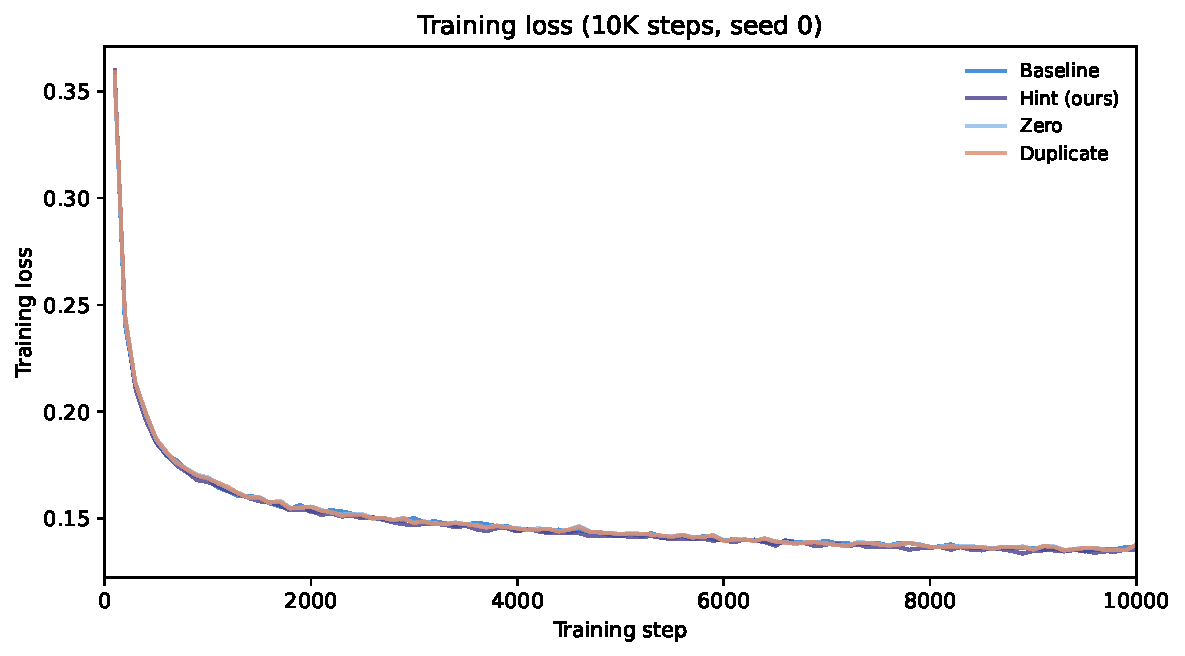
\includegraphics[width=0.5\linewidth]{figures/fig_training_loss_10k.pdf}%
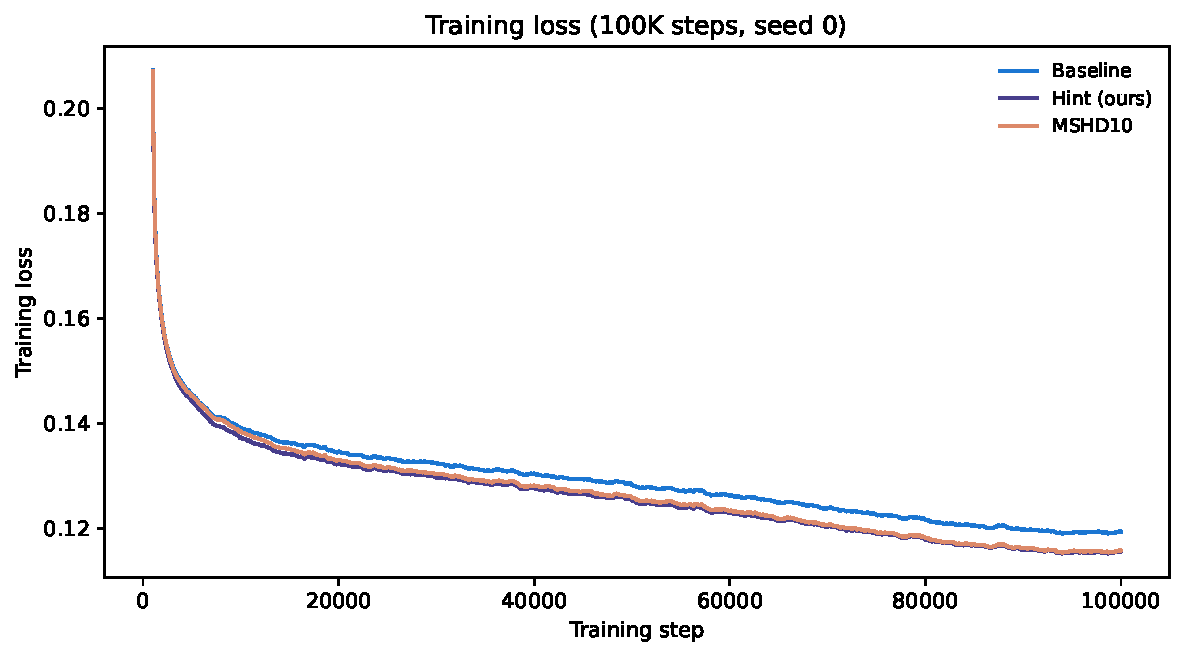
\includegraphics[width=0.5\linewidth]{figures/fig_training_loss_100k.pdf}
\caption{Training loss at 10K (left) and 100K (right) steps. HD10 maintains lower loss throughout. The baseline's eval collapse at 80K is not reflected in training loss.}
\end{figure}

\begin{table}[h]
\centering
\caption{Training loss means (5 seeds) vs.\ eval MASE. Training loss differences are small (1--2.4\%) while eval improvements are much larger (2.9--3.9\%), confirming hints act as a regularizer rather than simply improving optimization.}
\label{tab:trainloss}
\small
\begin{tabular}{lcccc}
\toprule
& \multicolumn{2}{c}{\textbf{10K steps}} & \multicolumn{2}{c}{\textbf{100K steps}} \\
\cmidrule(lr){2-3} \cmidrule(lr){4-5}
\textbf{Method} & \textbf{Train loss} & \textbf{Eval MASE} & \textbf{Train loss} & \textbf{Eval MASE} \\
\midrule
Baseline & .1364 & 0.862 & .1187 & 0.878 \\
\textbf{HD10 (ours)} & \textbf{.1350} & \textbf{0.837} & \textbf{.1159} & \textbf{0.844} \\
Zero & .1366 & 0.858 & .1187 & 0.894 \\
Duplicate & .1366 & 0.865 & .1190 & 0.886 \\
MSHD10 & --- & --- & .1146 & 0.838$^\dagger$ \\
\midrule
HD10 $\Delta$\% vs BL & $-1.0\%$ & $-2.9\%$ & $-2.4\%$ & $-3.9\%$ \\
Amplification & \multicolumn{2}{c}{$2.9\times$} & \multicolumn{2}{c}{$1.6\times$} \\
\bottomrule
\end{tabular}
\\[2pt]
{\footnotesize $^\dagger$MSHD10 eval mean over 3 available seeds (0, 2, 7).}
\end{table}

\section{Base Model Scale (46M Parameters)}
\label{app:base}

\begin{table}[h]
\centering
\small
\begin{tabular}{ccccc}
\toprule
\textbf{Seed} & \textbf{BL (46M)} & \textbf{HD10 (46M)} & \textbf{$\Delta$\%} & \textbf{Wins} \\
\midrule
0 & 0.8504 & 0.8520 & $-0.19\%$ & 52/95 \\
1 & 0.8473 & 0.8509 & $-0.42\%$ & 60/95 \\
42 & 0.8570 & 0.8417 & $+1.80\%$ & 59/93 \\
\bottomrule
\end{tabular}
\end{table}

Results are inconsistent at 46M scale, suggesting the benefit is specific to capacity-constrained models.

\section{FEV-Bench Evaluation}
\label{app:fevbench}

\begin{table}[h]
\centering
\caption{FEV-Bench results (100 task configurations). Geo = geometric mean MASE. SQL = squared log metric.}
\label{tab:fevbench}
\small
\begin{tabular}{lcccc}
\toprule
\textbf{Method} & \textbf{MASE (geo)} & \textbf{SQL (geo)} & \textbf{Wins/100} & \textbf{$\Delta$\% MASE} \\
\midrule
\textbf{HD10 (Ours)} & \textbf{1.253} & \textbf{1.657} & \textbf{72/100} & $+2.5\%$ \\
Baseline & 1.284 & 1.679 & --- & --- \\
\bottomrule
\end{tabular}
\end{table}

HD10 generalizes beyond GIFT-Eval to the FEV-Bench suite, winning 72 of 100 configurations with consistent improvement in both MASE and squared log metrics.

\section{Matched-Official Training Protocol (100K Steps)}
\label{app:matched_official}

\begin{table}[h]
\centering
\caption{Matched-official protocol: 10K warmup, 100K cosine schedule (matching the official Moirai-2 training configuration). Normalized MASE reported.}
\label{tab:matched_official}
\small
\begin{tabular}{lccccc}
\toprule
\textbf{Method} & \textbf{s0} & \textbf{s2} & \textbf{s7} & \textbf{Mean} & \textbf{$\Delta$\%} \\
\midrule
BL (10K warm) & 0.882 & 0.880 & 0.917 & 0.893 & --- \\
\textbf{HD10 (10K warm)} & \textbf{0.892} & \textbf{0.846} & \textbf{0.880} & \textbf{0.873} & $+2.3\%$ \\
\bottomrule
\end{tabular}
\end{table}

Under the official Moirai-2 training protocol (10K warmup steps, 100K total cosine schedule), HD10 still provides a 2.3\% improvement. The baseline's seed 7 (0.917) shows the late instability noted in \S5.5, which HD10 avoids (0.880).

\section{Leaderboard Context}
\label{app:leaderboard}

\begin{table}[h]
\centering
\caption{GIFT-Eval leaderboard context: normalized MASE (lower is better). HD10 Small (11.4M) outperforms Moirai 1.0 Large (311M) with $27\times$ fewer parameters.}
\label{tab:leaderboard}
\small
\begin{tabular}{lcc}
\toprule
\textbf{Model} & \textbf{Parameters} & \textbf{Normalized MASE} \\
\midrule
\textbf{HD10 Small (Ours)} & \textbf{11.4M} & \textbf{0.828} \\
Moirai-2 Small (retrained BL) & 11.4M & 0.862 \\
Moirai 1.0 Large & 311M & 0.875 \\
\bottomrule
\end{tabular}
\end{table}

HD10 at 11.4M parameters achieves 0.828 normalized MASE, surpassing Moirai 1.0 Large (311M, 0.875) with $27\times$ fewer parameters.

\end{document}
